
\documentclass[11pt,a4paper]{article}
\usepackage[left=2cm,right=2cm,top=2cm,bottom=3cm]{geometry}
\usepackage{amsmath,amsfonts,amsthm,amssymb,varioref,times, commath}
\usepackage{gensymb}
\usepackage{tikz}
\usepackage{textcomp}
\usepackage{hyperref}
\hypersetup{
 colorlinks=true,
 linkcolor=blue,
 filecolor=magenta, 
urlcolor=cyan,
}
\usepackage{lipsum}
\usepackage{epigraph}
%to resume numbering in a list
\usepackage{enumitem}
%----- arrows 
\usepackage{extarrows}

%    differential equatiosn 
\usepackage{diffcoeff}   %\diff[2]{x}{y}


%%%%%%pour ecrire en français avec les accents
\usepackage[utf8]{inputenc}
\usepackage[T1]{fontenc}
\usepackage{lmodern} % load a font with all the characters
\usepackage{units}
%%%%%%%Image-related packages
\usepackage{wrapfig}
\usepackage{float, graphicx}
\graphicspath{ {./img/} }
\usepackage{subcaption}
\usepackage[export]{adjustbox}

%%%%%%%pour faire des cadres
\usepackage{xcolor}
\usepackage{tcolorbox}
\usepackage{framed}
\usepackage{mdframed}


%%%%%%%chemistry frmulae
\usepackage{chemfig}
\usepackage{chemformula}
\usepackage[version=4]{mhchem}

% -------------- Circuits -------------------
\usepackage[european, straightvoltages]{circuitikz}

% Title & headers
\usepackage[explicit]{titlesec}
% Raised Rule Command:
% Arg 1 (Optional) - How high to raise the rule
% Arg 2 - Thickness of the rule
\newcommand{\raisedrulefill}[2][0ex]{\leaders\hbox{\rule[#1]{1pt}{#2}}\hfill}
\titleformat{\section}{\Large\bfseries}{\thesection. }{0em}{#1\,\raisedrulefill[0.4ex]{1pt}}

% pour ecrire sur +sieurs colonnes
\usepackage{multicol}
\setlength{\columnseprule}{0pt}
\setlength{\columnsep}{60pt}
% Fusion de lignes de tableaux.
\usepackage{multirow}
% Position verticale des lettres dans la ligne de tableau.
\usepackage{array}

% physics -----------------------------------------------------------
\newcommand{\To}{\longrightarrow}
\newcommand{\gpl}{\; g\cdot L^{-1}}
\newcommand{\gpmol}{\; g\cdot mol^{-1}}
\newcommand{\mpl}{\; mol\cdot L^{-1}}
\newcommand{\mps}{\; m\cdot s^{-1}}
\newcommand{\rps}{\; rad\cdot s^{-1}}
\newcommand{\kph}{\; km\cdot h^{-1}}
\newcommand{\mpss}{\; m\cdot s^{-2}}
\newcommand{\Dt}{\Delta t}
\newcommand{\vv}{\vec{v}}
\newcommand{\va}{\vec{a}}
\newcommand{\vp}{\vec{p}}
\newcommand{\vf}{\vec{F}}
\newcommand*{\Vf}[1]{\overrightarrow{F_\ensuremath{{#1}}}}
\newcommand{\es}[1]{\cdot10^{#1}}
\newcommand{\eng}[1]{\textcolor{purple}{(= #1})}
\usepackage{harpoon}
%\newcommand*{\vect}[1]{\overrightharp{\ensuremath{#1}}}
\newcommand*{\Vect}[1]{\overrightarrow{\ensuremath{#1}}}
\newcommand{\pfd}[1]{\sum \vec{F}_{ext_{#1}} &= \od{\vp_{#1}}{t} = m\cdot\va_{#1}}
\newcommand{\C}{\degree C}
\newcommand{\Delt}{\Delta t}

% --- Circuits ------------
\newcommand{\bipole}[1]{
\begin{circuitikz} \draw
(0,0) to[ #1 ] (2,0); 
\end{circuitikz} {\hspace{5mm}}}

% Chimie ---------------------------------
\newcommand{\oxo}{\ce{H3O+}_{(aq)}}
\newcommand{\eau}{\ce{H2O}_{(\ell)}}
\newcommand{\OH}{\ce{HO-}_{(aq)}}
\newcommand{\AH}{\ce{AH}_{(aq)}}
\newcommand{\A}{\ce{A-}_{(aq)}}
\newcommand{\MnO}{\ce{MnO_4^{-}}}
\newcommand{\conc}[1]{\left[{#1}\right]}
\newcommand{\couple}[2]{\ce{#1/#2}}


% Environnements ------------------------
\newcounter{exo}
\newenvironment{exo}[1][]
{\refstepcounter{exo} \begin{shaded}\noindent $\triangleright \quad$\textbf{Exercice~\theexo. #1} } { \end{shaded}}
\newenvironment{eg}
{\begin{shaded} \textbf{Exemple:} } { \end{shaded}}

\newenvironment{defn}[1]
{\begin{leftbar}\noindent \textbf{Définition :\textit{ \quad #1}} } { \end{leftbar}}

%\newenvironment{rmrq}
%{\begin{shaded} \textbf{Remarque.\quad } \itshape } { \end{shaded}}
\newenvironment{rmrq}
{\begin{mdframed}[backgroundcolor=blue!10, linewidth=0pt] \textbf{Remarque.\quad } \itshape } { \end{mdframed}}

\newenvironment{python}
{\begin{shaded} \textbf{A faire en PYTHON}\\ \itshape } { \end{shaded}}

% Shading colour -----------------------------
\definecolor{shadecolor}{gray}{0.9}

\date{}
\author{}

\renewcommand*\contentsname{Résumé}









% Title & headers 
\usepackage{fancyhdr}
\pagestyle{fancy}
\fancyhf{}
\lhead{SciPhy : Terminale spé}
\rhead{$\Phi $ - 9 : Fluides}
\chead{2020-28}
\rfoot{Page \thepage}
\lfoot{\textcopyright\; S Zayyani}
\renewcommand{\footrulewidth}{0.1pt}% default is 0pt

\title{\large Physique - Chapitre 9 \\ \LARGE  La mécanique des fluides}
\date{}
\author{}

\setlength{\parindent}{0mm}
\setlength{\parskip}{2mm}

%%%%%%%%%%% For wrapfigure 
\setlength{\intextsep}{3pt}%
\setlength{\columnsep}{3pt}%



\begin{document}
\maketitle
\vspace{-1cm}
\begin{tcolorbox}[title=Notions de la classe de première à rappeler]
Pression ; loi fondamentale de la statique des fluides incompressibles ; masse volumique ; Loi de Boyle-Mariotte
%\tcblower
\end{tcolorbox}
\tableofcontents

\section{Rappels : Pression}
Comme vous avez vu en seconde ou en première, une pression\eng{pressure} est une \textbf{force pressante $F$ repartie sur une surface} $S$ : donné par la relation 
\[ P = \dfrac{F}{S} \quad \quad  où \quad  \quad 
\begin{cases}
     p \rightarrow \text{pression }(Pa) \\
     S \rightarrow \text{aire de la surface }(m^2) \\ 
     F \rightarrow \text{force pressante en }(N) 
\end{cases} 
\]
L'unité légale de la pression est le \textit{pascal (Pa)}. C'est une très petite unité (imaginez la poids d'une masse de $10\,g$ repartie sur une surface de $1\;m^2$); et donc nous avons l'habitude d'utiliser d’autres unités, ou des multiples du pascal.  Par exemple, la pression atmosphérique est d’ordre de $10000\; Pa$, on utilise donc, soit l’\textit{hectopascal} ($hPa = 10^2\; Pa)$ ou le \textit{Bar} ( $1\; bar = 10^5\; Pa $).  

\subsection*{Loi de Boyle-Mariotte}
Pour une température constante, et une quantité de gaz fixée, le produit de la pression $p$ par le volume $V$ qu’occupe un gaz est constante. C’est-à-dire : 
\[ P\cdot V = constante\]

\subsection*{Pression dans un fluide}

\begin{wrapfigure}[10]{r}{0.35\textwidth}
\centering
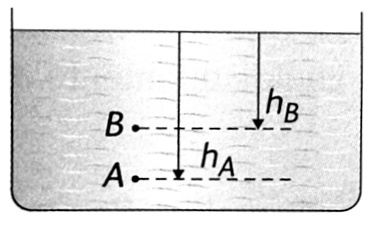
\includegraphics[width=0.9\linewidth]{imgs/p9/p10-1.jpg}
\caption{}
\end{wrapfigure}

Un objet immergé dans un liquide est soumis à une force pressante exercée par le liquide. La pression qui en résulte dépend de la profondeur d’immersion.

La différence de pression $\Delta p = p_A - p_B$  entre deux points $A$ et $B$ situés à des profondeurs $h_A$  et $h_B$ dans un fluide caractérisé par la masse volumique $\rho$, est proportionnelle à la différence de profondeur $h_A - h_B$ ∶ 

\[ \Delta p = p_A - p_B = \rho g \left( h_A - h_B \right) \]

Cette relation s'appelle la \textbf{loi des de la statique des fluides incompressibles}, ou la loi de l'hydrostatique.

Dans le cas de l’eau donc, la pression augmente de 1 bar tous les 10 m. Dans un liquide de masse volumique $\rho$ , la pression du fluide à une profondeur de $h$ s’écrit : $p = p_{atm} + \rho g h $

\section{Poussée d'Archimède : conséquence de la pression atmosphérique}
\begin{quote}
    « Tout corps plongé dans un fluide au repos, entièrement mouillé par celui-ci ou traversant sa surface libre, subit une force verticale, dirigée de bas en haut et opposée au poids du volume de fluide déplacé. Cette force est appelée poussée d'Archimède. Elle s'applique au centre de masse du fluide déplacé, appelé centre de poussée. »
\end{quote}

\begin{wrapfigure}[14]{r}{0.55\textwidth}
\centering
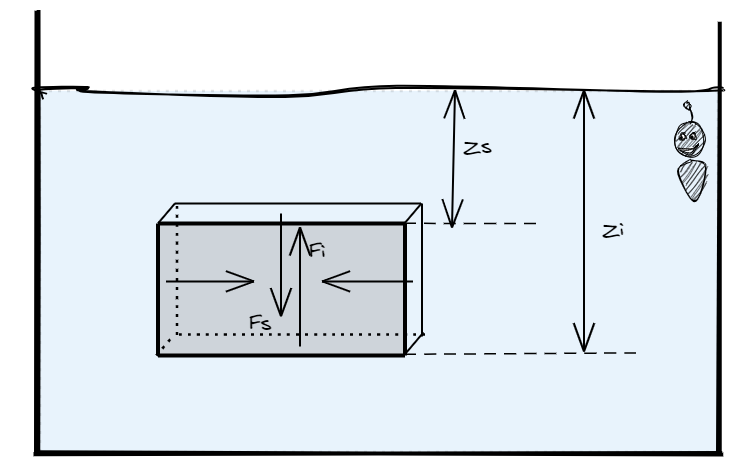
\includegraphics[width=0.95\linewidth]{imgs/p9/archimede2.png}
\caption{}
\label{fig:archimede}
\end{wrapfigure}
Considérons un cube de volume $V$ de surface $S$ de chaque face de longueur $h$, plongé dans un fluide avec une masse volumique $\rho_f$. La surface supérieure du cube est à un profondeur de $z_s$ et la surface inférieure à une profondeur de $z_i$.

Chaque face du cube est assujettie à un pression, due au poids du fluide, au dessus de cette surface. Nous pouvons déjà faire une simplifications : les pressions sur les faces verticales s'annulent, étant égales et opposées. 

En revanche, la pression sur la surface supérieure (et donc la force pressante correspondant) est plus faible que la pression sur la surface inférieure, ( cette dernière étant plus profonde dans le fluide) : 
\newpage
Faisons donc un petit bilan des forces : 
\begin{align*}
    p_s &= \dfrac{F_s}{S} = \dfrac{m_f_s\cdot g}{s} = \dfrac{\left(S\cdot z_s\cdot\rho_f\right)\cdot g}{S} =\rho_f\cdot g\cdot z_s\\
    p_i &= \dfrac{F_i}{S} = \dfrac{m_f_i\cdot g}{s} = \dfrac{\left(S\cdot z_i\cdot\rho_f\right)\cdot g}{S} =\rho_f\cdot g\cdot z_i
\end{align*}

La différence de pression entre les deux surfaces est donc : 
\begin{align*}
    \Delta p &= p_i - p_s \\
        &= \rho_f\cdot g\left(z_i - z_s\right) \tag{1}\\
        &=\rho_f\cdot g\cdot h
\end{align*}

On remarque qu'une simple analyse des pressions sur les facettes de l'objet nous donne (1) la loi de l'hydrostatique, vue précédemment. 

La poussée d'Archimède\eng{Archemides principle, buoyancy force}  est une force (notée $\Pi_A$), et plus précisément la force du fluide sur l'objet, autrement dit c'est la force due à cette différence de pression $\Delta P$ : 
\begin{align*}
    \Pi_A &= \Delta P\cdot S \\
        &= \rho_f\cdot g\cdot h\cdot S \\
     \Pi_A   &= \rho_f\cdot g\cdot V \tag{2}
\end{align*}

Il y a une façon très simple d'interpréter l'expression (2) : la norme de la poussée d'archimède est est l'équivalente du poids du fluide déplacée par le cube par son immersion dans le fluide. C'est justement la raison pour laquelle cette force est attribuée au savant grec, d'après son célèbre moment ``Euréka!'', après s'être plongé dans un bain public et voyant l'eau qui se déborde, déplacée par son corps. 

La \textbf{forme vectorielle} de la poussée d'archimède est donnée par 
\[\overrightarrow{\Pi_A} = - \rho_f\cdot V \cdot \Vec{g} \tag{3} \]
car cette force est, par définition, opposée au poids de l'objet. 

\begin{exo}
\begin{wrapfigure}[11]{r}{0.35\textwidth}
\centering
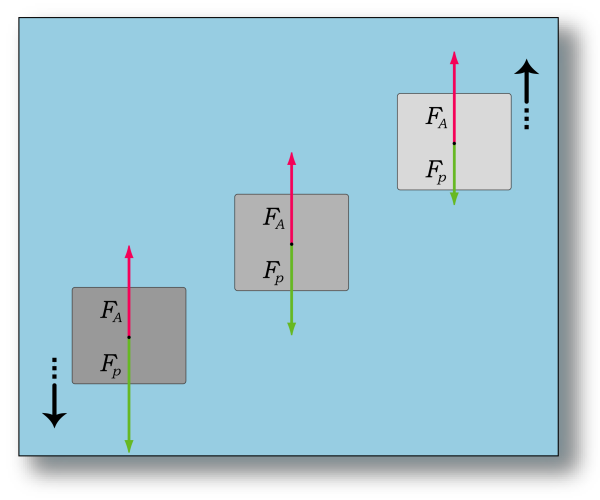
\includegraphics[width=0.95\linewidth]{imgs/p9/archimede.png}
\end{wrapfigure}
Justifier le fait qu'un objet ayant une densité $d>1$ coule, et un ayant une densité $d<1$ flotte. 
\vspace{5cm}
\end{exo}

\begin{exo}
Justifier que la fonte d'un morceau de glace pure flottant sur de l'eau pure se produit sans changement de niveau de l'eau.
\vspace{3.5cm}

\end{exo}
\begin{exo}
Déterminer la masse volumique de glace étant donné que le volume immergé représente près de 90\% du volume total d'un iceberg. 
\vspace{4cm}
\end{exo}

\begin{exo}
Un cylindre en Fer $\rho_{Fe} = 7,874\,g\cdot cm^{-3}$ est placée dans un bain de mercure $\rho_{Hg} = 13,546\,g\cdot cm^{-3}$. Déterminer la portion du cylindre qui reste émergée. 
\vspace{4cm}
\end{exo}

\section{L'écoulement d'un fluide}

\subsection{Différents régimes}

Pour commencer une étude de la mécanique des fluides il faut d'abord limiter le champ d'étude, car le domaine est beaucoup trop vaste pour une classe de terminale. Nous nous limitons donc aux \textbf{fluides non-compressibles}, ce qui élimines les gaz et donc nous laisse avec la plupart des liquides.  

D'autre part nous allons nous limiter au \textbf{régime permanent d'écoulement}. Un fluide peut s'écouler dans des différentes régimes. On fait donc la distinction entre ceux-là : 
\begin{itemize}
    \item Régime \textbf{permanent}\eng{laminar flow} (ou régime stationnaire) est quand que les conditions d'écoulement ne changent pas. Alors, la vitesse d'un point quelconque ne dépend pas du temps, mais uniquement de la position du point. 
    \item Régime \textbf{turbulent}\eng{turbulent flow} est cas contraire d'un écoulement permanent, caractérise par le mouvement irrégulier et erratique des particules du fluide. 
    \item Régime \textbf{transitoire} est le régime de transition entre un régime permanent et un régime turbulent. 
\end{itemize}

\begin{figure}[H]
\centering
\begin{subfigure}{.25\textwidth}
  \centering
  % include first image
  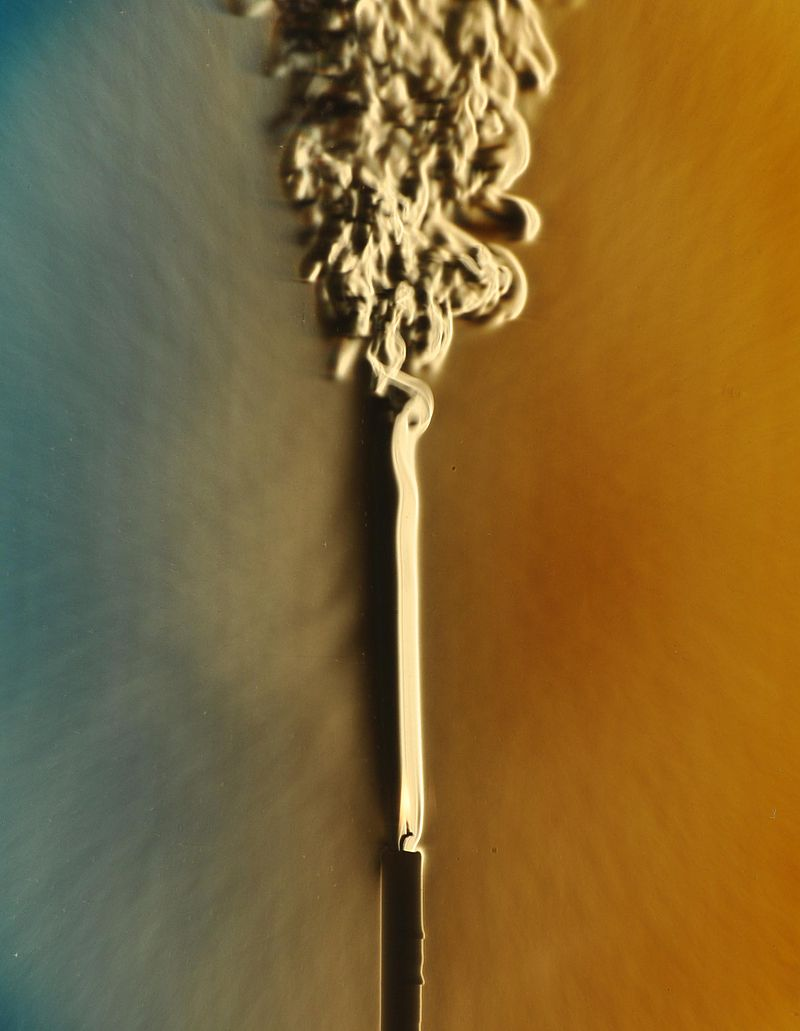
\includegraphics[width=.95\linewidth]{imgs/p9/flows.jpg}  
\end{subfigure}
\begin{subfigure}{.35\textwidth}
  \centering
  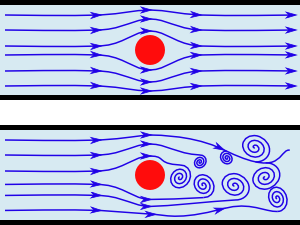
\includegraphics[width=.95\linewidth]{imgs/p9/flows.png}  
\end{subfigure}
\begin{subfigure}{.37\textwidth}
  \centering
  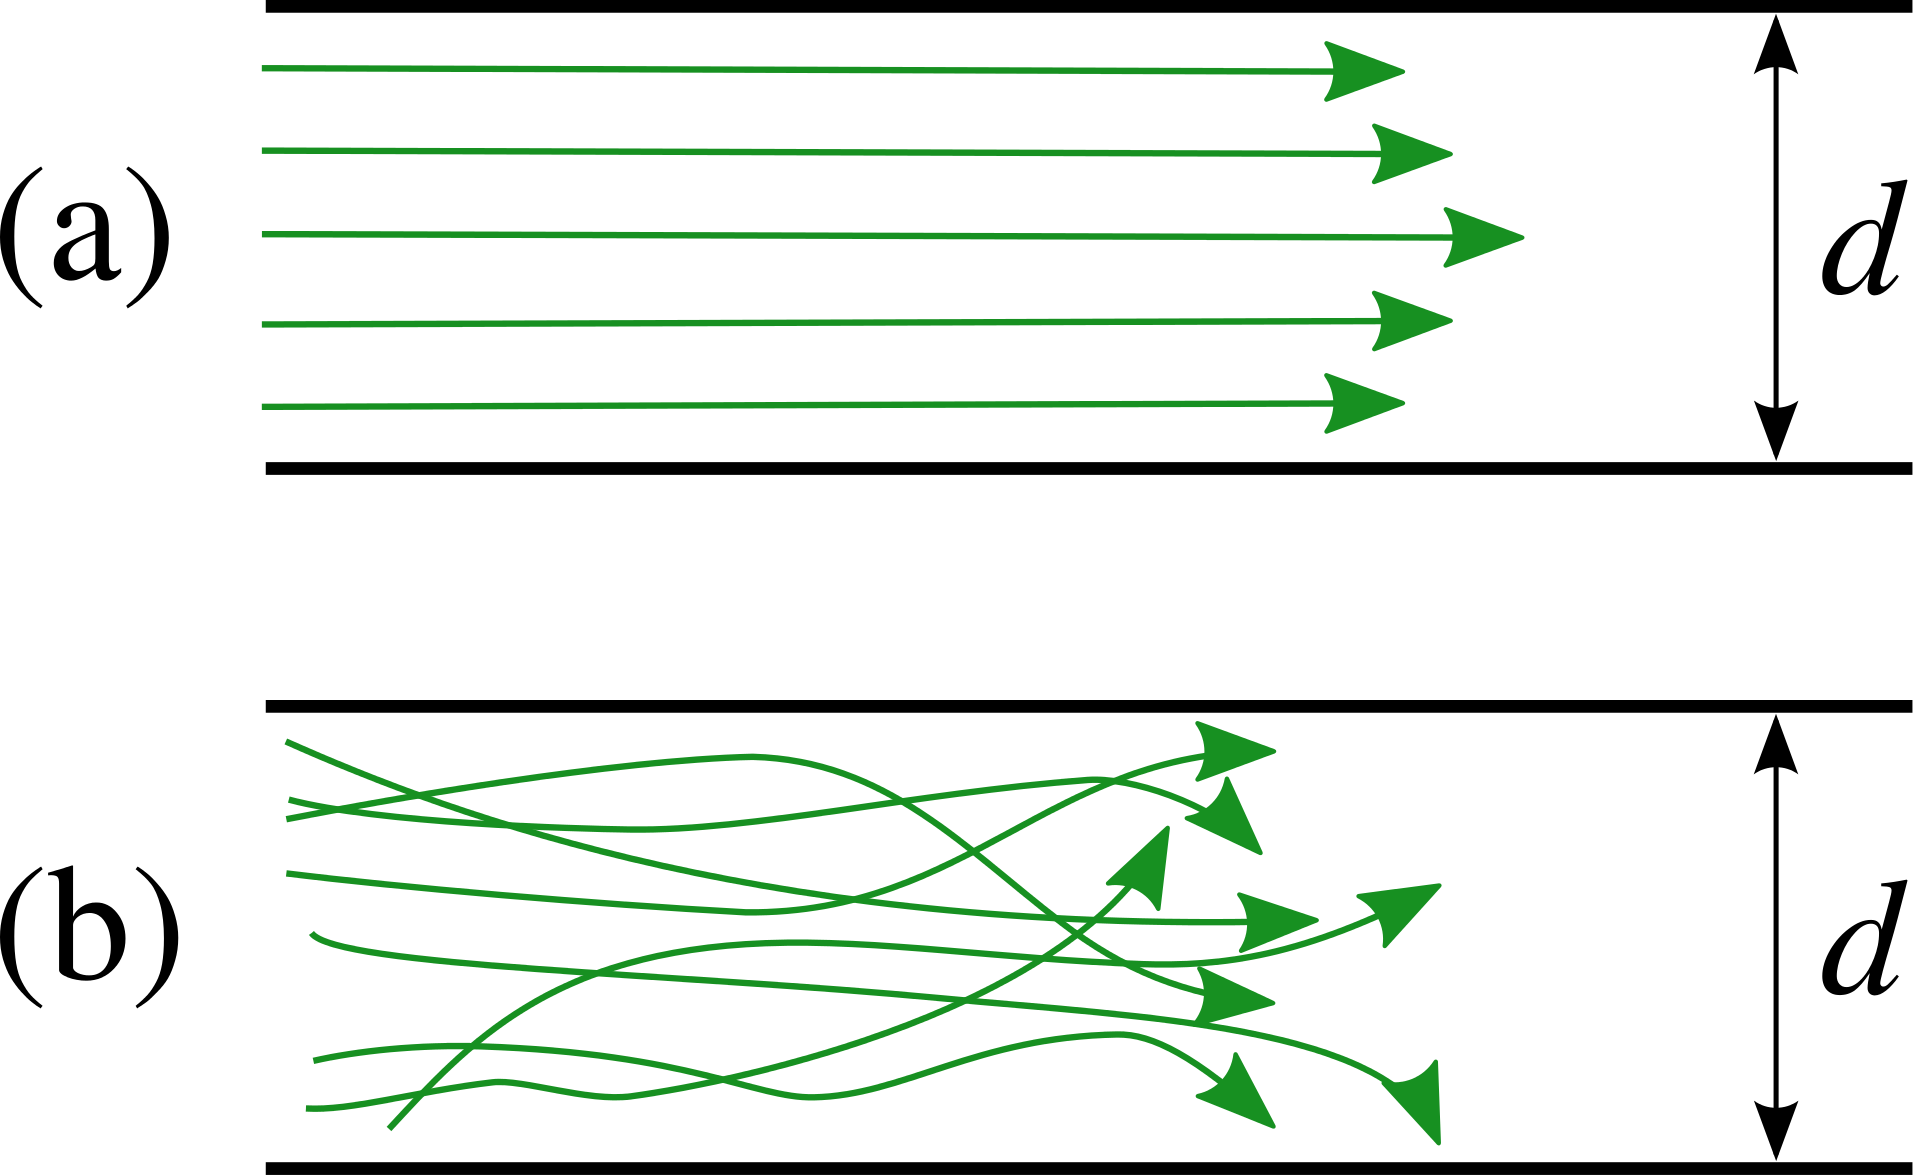
\includegraphics[width=.95\linewidth]{imgs/p9/flows2.png}  
\end{subfigure}
\caption{Trois exemples d'écoulements laminaires et turbulents.}
\end{figure}

Il ne faut pas oublier qu'en physique nous construisons des modèles, et que ces modèles \textit{ressemble} à la réalité, mais souvent avec moins de complexité. Bien sur, la plupart des liquides sont compressibles, même l'eau, mais dans des conditions normales, on peut les considérer comme les fluides parfaits, et donc notre modèle est suffisant pour un début. 

\subsection{Vitesse d'écoulement \& et section droite}

\begin{defn}{Débit volumique\eng{volumetric flow rate}}
\begin{itemize}
    \item Le débit volumique est une mesure du volume de fluide qui passe par une surface $S$ pendant une période $\Dt$. 
    \item Il est donné par la relation : 
    \[   D_V = \dfrac{V}{\Dt}  
    \quad \quad  où \quad  \quad 
    \begin{cases}
    D_V \rightarrow \text{débit en }(m^3\cdot s^{-1}) \\
    V \rightarrow \text{volume en }(m^3) \\
     \Dt \rightarrow \text{durée }(s) \\ 
    \end{cases}
    \]
\end{itemize}
\end{defn}

Si l'on considère un écoulement dans un conduit, on peut considérer la \textbf{section droite $S$} de la canalisation, c'est-à-dire l'intersection du plan perpendiculaire au vecteur-vitesse du fluide, et la canalisation. 

\begin{figure}[H]
    \centering
    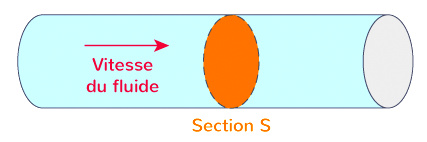
\includegraphics[width=0.7\linewidth]{imgs/p9/sectionTube.jpg}
    \caption{}
\end{figure}

\begin{defn}{Vitesse d'écoulement}
\begin{itemize}
    \item Il s'agit de la vitesse de déplacement d'une particule, ou d'un point, du fluide à un instant donné. 
    \item Elle est donnée par la relation : 
    \[v = \dfrac{D_V}{S}
    \quad \text{où} \begin{cases}
    v \rightarrow \text{vitesse d'écoulement en }(\mps) \\
    D_V \rightarrow \text{débit volumique en }(m^3\cdot s^{-1}) \\
    S \rightarrow \text{section droite en }(m^2) 
    \end{cases}
    \]
\end{itemize}
\end{defn}

\begin{exo}
De l'eau coule dans une canalisation cylindrique de $5,0\,cm$ de diamètre, avec un débit $50\,m^3\cdot s^{-1}$. Déterminer la vitesse vitesse d'écoulement. 
\vspace{5cm}
\end{exo}


\subsection{Principe de continuité \& la loi de conservation du débit}

\begin{wrapfigure}[6]{r}{0.4\textwidth}
\centering
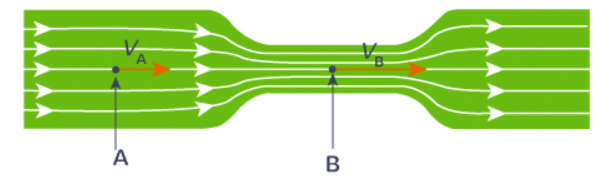
\includegraphics[width=0.95\linewidth]{imgs/p9/tubechange.jpg}
\caption{}
\label{fig:tubechange}
\end{wrapfigure}
Le principe fondamentale des fluides est une conséquence de la \textbf{conservation de la masse} : Quand un fluide s’écoule, il n’y a ni apparition, ni disparition de matière. Autrement dit à travers chaque section de l’écoulement s’écoule la même masse $\Delta M$ de fluide pendant la même durée $\Delta t$ : c'est le \textbf{principe de continuité}. 


Il y a bien sur des conséquences visibles de ce principe, notamment la changement de vitesse du débit en fonction de la section d'écoulement. Considérons un écoulement dans des conduits ou la section change, comme la figure (\ref{fig:tubechange}). Le principe de continuité, exige une conservation du débit volumique lors du passage dans le tuyau. Entre le point $A$ et $B$ donc, on peut écrire : 
\begin{align*}
    D_V(A) &= D_V(B) \\
    v_A\cdot S_A &= v_B\cdot S_B \\
    v_A &= v_B\left(\dfrac{S_B}{S_A} \right)
\end{align*}

L'interprétation de cette petite démonstration est simple, et même plutôt intuitive : un fluide accélère quand il passe dans une partie plus étroite de la canalisation, et ralentit quand la canalisation s'ouvre. 

\begin{exo}
Un fluide coule avec une vitesse $v$ dans un tuyau avec une section de rayon $r$. Déterminer sa vitesse $v'$ en passant dans une autre partie ayant un rayon $r'$ deux fois plus grand que la partie précédente. 
\vspace{3cm}
\end{exo}

\subsection{Énergies volumiques}

Tout ce que l'on a vu cette année en mécanique se relève de la mécanique du point. La raison est simple, en assimilant un objet à un point l'analyse de son mouvement est plus simple et plus facile, tout en restant parfaitement valable pour une étude générale de son mouvement. Avec les fluides ceci n'est pas aussi facile; comment assimiler un fluide en écoulement à un point. Nous parlons, en revanche, des volumes de fluides qui se déplacent, ou une surface parcourue par un fluide. 

On peut donc parler d'une ``particule'' de fluide en désignant un cube élémentaire, de longueur $a$ d'un coté. Son volume est donc $a^3$, et chaque facette aura une aire de $a^2$. Cela nous permet alors de définir son énergie cinétique et ses énergies potentielles, ou plus précisément ses énergies mécaniques volumiques. 

Pour une particule d'une fluide ayant une masse volumique $\rho$ : 
\begin{itemize}
    \item \textbf{Energie cinétique} : $E_c = \dfrac{1}{2}mv^2 = \dfrac{1}{2}\rho a^3 v^2 = a^3\cdot e_c$, où $e_c=\dfrac{1}{2}\rho v^2 $ est l'\textbf{énergie cinétique \textit{volumique}} du fluide. 
    \item \textbf{Energie potentielle de pesanteur} : $E_{pp} = mgz = \rho a^3 g z = a^3\cdot e_pp$, où $e_{pp} = \rho g z $ est l'\textbf{énergie potentielle de pesanteur \textit{volumique}} du fluide. 
\end{itemize}

L'intérêt de ces \textbf{``énergies volumique''\eng{energy density}} est de trouver des grandeurs qui caractérisent le fluide, indépendemment de la quantité ou volume considéré. 

Mais, c'est bien possible de s'interroger sur le rôle joué par la pression dans cette affaire. Si c'est votre car, alors vous avez de bons instincts, car la pression est une des grandeurs d'état d'un fluide; jetons donc un coup d'\oe il rapide dans cette direction. 

L'unite de la pression est le \textit{Pascal}, qui, à partir de la définition de la pression est une unité composée :  $Pa = N\cdot m^{-2}$. 

Mais le \textit{Newton}, aussi, est une unité composée (et donc à partir du PFD) $N = Kg\cdot \mpss$. 

Nous avons donc : 
\begin{align*}
    Pa &= N\cdot m^{-2} \\
    &= Kg\cdot \mpss\cdot m^{-2} \\
    &= Kg\cdot m^2 \cdot s^{-2}\cdot m^{-3} \\
    &= J\cdot m^{-3} \quad (\text{le joule, à partir de l'énergie cinétique)} \tag{4}
\end{align*}

\begingroup 
\setlength{\columnsep}{15pt}% 
\setlength{\intextsep}{-10pt}% 
\begin{wraptable}[8]{r}{0.35\linewidth} 
\begin{rmrq} 
\small{Cela ne doit pas nous étonner, car la pression est une force repartie sur une surface. Cette même force/pression est responsable du déplacement du fluide, et donc quand nous avons un déplacement du à une force ... il y a du travail! Vous devez donc pouvoir voir dans l'expression de l'énergie mécanique d'un fluide, un résultat du théorème de l'énergie cinétique ! } 
\end{rmrq} 
\end{wraptable} 

Hmmm! On vient de montrer (4) donc, que la pression est homogène à une énergie volumique! 

Pour calculer l'énergie mécanique volumique d'un fluide il faut donc 
\begin{align*}
    E_{m,V} &= E_{c,V} + E_{pp,V} + E_{P,V} \\
    E_{m,V} &=  \dfrac{1}{2}\rho v^2 + \rho g z + p \tag{5}\\
    E_{m,V} &=  \rho \left(\dfrac{1}{2}v^2 + g z \right) + p \tag{6}
\end{align*} 

\endgroup
\vspace{0.3cm}
\section{Lois de la mécanique des fluides}

Comme beaucoup de lois de physique, dans de divers domaines, le principe fondamental à l'origine des choses est la \textbf{conservation de l'énergie}. Comme déjà dit, précédemment, nous allons nous limiter ici aux \textbf{fluides parfaits}, avec la précision qu'il s'agit des fluides avec une \textbf{viscosité négligeable}, la viscosité étant un une mesure des forces de \textbf{résistance à l'écoulement} (frottement) à l'intérieur du fluide. 

\subsection{Relation de Bernoulli}
Dans le cas d'un fluide parfait, l'énergie mécanique volume d'un fluide se conserve. Considérons alors un cas quelconque, comme dans la figure (\ref{fig:bernoulli}). 

\begin{figure}[H]
    \centering
    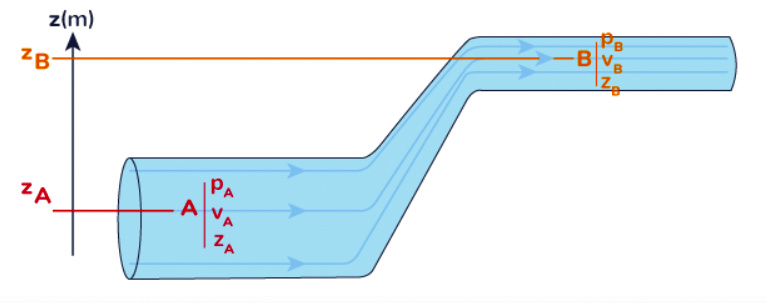
\includegraphics[width=0.75\linewidth]{imgs/p9/bernoulli.jpg}
    \caption{}
    \label{fig:bernoulli}
\end{figure}

A partir du principe de la conservation d'énergie on obtient la relation suivante, dite la \textbf{relation de Bernoulli}, nommée d'après \textbf{Daniel Bernoulli (1738)} : 

\begin{align*}
    E_{m,V}(A) &= E_{m,V}(B) \\
    \dfrac{1}{2}\rho v_A^2 + \rho g z_A + p_A &= \dfrac{1}{2}\rho v_B^2 + \rho g z_B + p_B \tag{7}
\end{align*}

La forme courante de la relation de Bernoulli, est grâce à \textbf{Léonard Euler (1752)}, et est souvent donnée aussi sous forme 

\[ \dfrac{v^2}{2} + \dfrac{p_1}{\rho}+ gh = constante \tag{9}
\]
\newpage
\begin{exo}

\begin{wrapfigure}[8]{r}{0.45\textwidth}
    \centering
    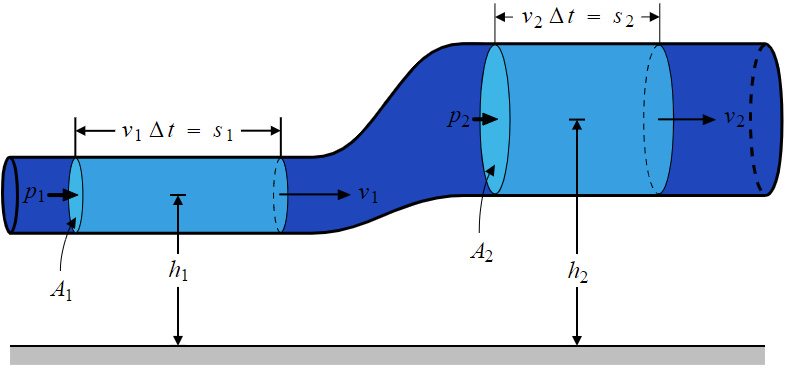
\includegraphics[width=0.98\linewidth]{imgs/p9/bernoulli1.jpg}
\end{wrapfigure}
Servez-vous de la figure ci-contre afin de retrouver l'expression de la relation de Bernoulli (9), à partir du théorème de l'énergie cinétique. Aide :  la pression et la gravitation sont les deux forces qui travaillent. 
\vspace{9cm}
\end{exo}

\begin{exo}
Considérons un conduit en forme de la figure (\ref{fig:bernoulli}). Déterminer la pression au point $A$, si : $ v_A = 2,0\mps \quad v_B=0,5\mps\quad z_A=0,5\,m \quad z_B=2,50\,m\quad p_B=6,0\,bar$. 
\vspace{5cm}
\end{exo}

\begin{rmrq}
Comme dans l'exercice précédent, nous pouvons arriver à la relation de Bernoulli à partir de différents type de raisonnement. Voici un autre exemple (simplifié), où l'on arrive à la relation (9) à partir de la deuxième loi de Newton, notre ami le PFD. Afin de simplifier la démonstration nous considérons le cas d'un conduit horizontale, où il n'y a pas de changement de hauteur. 

D'après le PFD, pour une particule de fluide de densité $\rho$ et de section $A$, et d'une longueur $\dl x$, subissant une pression $p$ : $ m\diff{v}{t} = \sum F$

\begin{minipage}{0.7\textwidth}
\begin{align*}
    m\diff{v}{t} &= \sum F \\
    \rho\cdot A\cdot \dl x \cdot\diff{v}{t}&= -A \dl p \\
    \rho\cdot\diff{v}{t}&= -\diff{p}{x} \\
    \rho\cdot\diff*{\left(\dfrac{v^2}{2}\right)}x &= -\diff{p}{x} \\
\end{align*}
\end{minipage}
\begin{minipage}{0.25\textwidth}
\begin{framed}
Rappel : 
\begin{align*}
    \diff{v}{t} &= \diff{v}{x}\diff{x}{t}\\
    &= v\diff{v}{x}\\
    &= \diff*{\left(\dfrac{v^2}{2}\right)}x
\end{align*}
\end{framed}
\end{minipage}

On regroupe tous les termes assujettis à une dérivé par rapport à $x$ : 
\[    \diff*{\left(\dfrac{\rho v^2}{2} + p\right)}{x} &= 0 \]
ce qui implique que : 
\begin{align*}
    \dfrac{\rho v^2}{2} + p &= constante \\
    \dfrac{v^2}{2} + \dfrac{\rho}{p} &= constante
\end{align*}
Et nous retrouvons alors la relation de Bernoulli. 
\end{rmrq}

Nous pouvons étudier, ou \textit{jouer}, un peu plus avec cette relation afin de mieux voir ses conséquences. Considérons le cas où $v=0$ alors 
\[ p +\rho g h = constante\]
mais nous connaissons cette relation : c'est la \textbf{loi de l'hydrostatique} (une appellation donc parfaitement logique car un fluide ayant une vitesse nulle est statique.) 

Un autre phénomène, expliqué par la relation de Bernoulli, est le \textbf{principe de Torricelli}, établissant une relation de proportionnalité entre la vitesse d'écoulement d'un fluide la hauteur de fluide située au-dessus de l'ouverture par laquelle il s'échappe du cylindre qui le contient : $v^2 = \sqrt{2gh}$. 

\begin{exo}

\begin{wrapfigure}[8]{r}{0.25\textwidth}
    \centering
    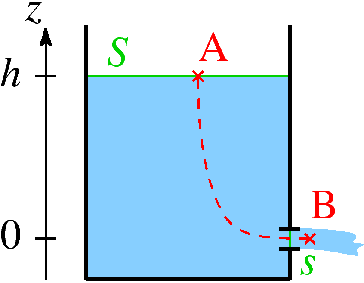
\includegraphics[width=0.9\linewidth]{imgs/p9/Torricelli.png}
\end{wrapfigure}
Comme dans le figure ci-contre, on note $A$ un point choisi au hasard sur la surface libre du liquide et $B$ un point pris au niveau du jet libre généré par le trou. Montrer, en utilisant la relation de Bernoulli, que $v_B^2=\sqrt{2gh}$
\vspace{5cm}
\end{exo}

\subsection{L'effet Venturi}

Un autre phénomène intéressant et connu en mécanique de fluide, que l'on peut expliquer grâce à la relation de Bernoulli est un effet connue sous le nom de ``L'effet Venturi''. 

\begin{figure}[H]
    \centering
    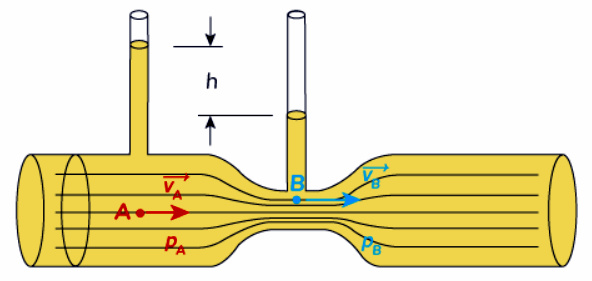
\includegraphics[width=0.6\linewidth]{imgs/p9/venturi.jpg}
    \caption{Une visualisation de l'effet Venturi}
    \label{fig:venturi}
\end{figure}

L'effet venturi est le phénomène par lequel la \textbf{pression dans un conduit diminue quand la vitesse d'écoulement augment, }comme dans la figure (\ref{fig:venturi}), autrement dit, la pression dans le conduit est inversement proportionnelle à la section droite de le conduit. 

\begin{exo}
Mettre en évidence l'effet Venturi, à partir de la relation de Bernoulli. 
\vspace{5cm}
\end{exo}

Il existe de nombreuse exploitation de ce phénomène, comme dans la figure (\ref{fig:venturiapp}).

\begin{figure}[H]
\centering
\begin{subfigure}{.47\textwidth}
  \centering
  % include first image
  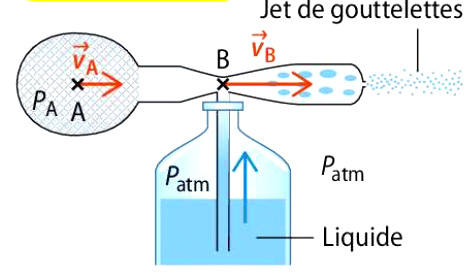
\includegraphics[width=.95\linewidth]{imgs/p9/parfum.jpg}  
\end{subfigure}
\begin{subfigure}{.4\textwidth}
  \centering
  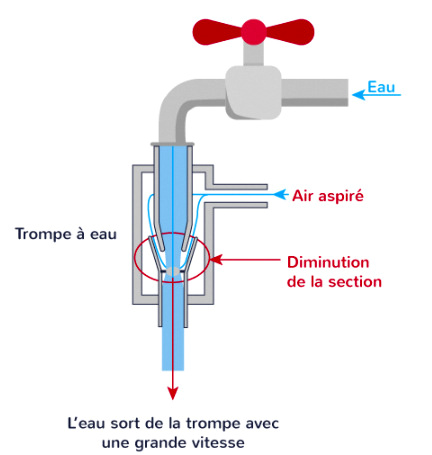
\includegraphics[width=.95\linewidth]{imgs/p9/trompe.jpg}  
\end{subfigure}
\caption{Deux applications de l'effet Venturi.}
\label{fig:venturiapp}
\end{figure}

\end{document}